\subsubsection{Use Case 2: Create an UNESCO Term Status}\label{ssec:UseCase2-Unesco Thesaurus}

This use case is part of the scenario of managing an ontology, and it captures the special behavior of retrieving resources that lack the requested column property. This condition may either be a deliberate choice by users—as they aim to create the desired property values from scratch—or an accident due to a false configuration. In either way, the prototype should react appropriately to handle this case.


In this use case, the \tracknshrink{UNESKOS} ontology \parencite{PastorSanchez2015} acts as the underlying graph. \mbox{\tracknshrink{UNESKOS}} is the \acrshort*{SKOS}\footnote{\acrfull*{SKOS} is a W3C recommendation \textit{“[\textellipsis{}] designed for representation of thesauri, classification schemes, taxonomies, subject-heading systems, or any other type of structured controlled vocabulary”} \parencite[455]{Garoufallou2015}.} version of the \tracknshrink{UNESCO} thesaurus.\footnote{The \textit{“\tracknshrink{UNESCO} Thesaurus is a controlled and structured list of terms used in subject analysis and retrieval of documents and publications in the fields of education, culture, natural sciences, [\textellipsis{}]”} \parencite{UNESCO}.} The content of this vocabulary is built hierarchically, and its first level consists of seven major subject domains\footnote{These are education, science, culture, social and human sciences, information and communication, politics, law and economics, and countries and country groupings. See \url{http://skos.um.es/unescothes/CS000/html}.} containing over 4,000 terms (or concepts). For example, the concept \textit{Deforestation} can be retrieved when traversing the graph by:\\
\centerline{\textit{\tracknshrink{UNESCO} Thesaurus} \textrightarrow {} \textit {Politics, law and economics} \textrightarrow{} \textit{Agriculture} \textrightarrow{} \textit{Deforestation}}



\vspace*{\baselineskip}

\noindent \textsc{Outline}\\
\noindent Unlike the previous use case, \tracknshrink{UNESKOS} terms do not contain a status property. However, it may be the user’s desire to define status values for resources from scratch. Since all \tracknshrink{UNESKOS} resources lack the demanded \acrshort{vs}\texttt{term\_status} property, all resources should be placed in a fallback column labeled \textit{no property}. From there, a user can create new column values and start to assign the resources to the desired column position. Moreover, due to the vast number of \tracknshrink{UNESKOS} terms, an implicit card limit should be set to prevent a stalling behavior of the user’s browser.


\vspace*{\baselineskip}

\noindent \textsc{Board Component Resources}\\[-1.5em]

\noindent \hangindent=1.7cm \textit{Cards.}\tabto{1.7cm} Each term defined within the \tracknshrink{UNESCO} vocabulary refers to a \acrshort{skos}\texttt{Concept}. Thus, each card represents a \acrshort{skos}\texttt{Concept}.\\[-1.5em]

\noindent \hangindent=1.7cm \textit{Columns.}\tabto{1.7cm} As stated above, the \tracknshrink{UNESKOS} graph does not contain a status property; however, this scenario utilizes the status vocabulary \acrshort{vs}\texttt{term\_status}, similar to the first use case\\[-1.5em]

\noindent \hangindent=1.7cm \textit{Lanes.}\tabto{1.7cm} Every \tracknshrink{UNESKOS} term has a broader umbrella term (i.e., a hyponym) within the hierarchical structure of the thesaurus (i.e., \acrshort{uneskos}\texttt{memberOf}). For example, the semantic triple for the concept \textit{Deforestation} is:\\
\centerline{\textit{Deforestation} \textrightarrow{} \textit{\acrshort{uneskos}\texttt{memberOf}} \textrightarrow{} \textit{Agriculture}}\\
Thus, \textit{Agriculture} as a single swimlane groups a variety of related \tracknshrink{UNESKOS} terms.


\vspace*{\baselineskip}
\newpage

\noindent \textsc{Card Component Resources}\\
\noindent The card titles correspond to the \tracknshrink{UNESKOS} term labels. However, unlike within the \acrshort*{FOAF} vocabulary, \tracknshrink{UNESKOS} terms do not contain any descriptive property. This means that all cards initially contain only their title and their corresponding \acrshort*{URI} since both items are mandatory for every card. Nevertheless, moving a card into a new column generates a timestamp property, which is also depicted on the corresponding card.


\vspace*{\baselineskip}

\noindent \textsc{Mockup}\\
\noindent \autoref{fig:RMB Use Case 2} provides a mockup of the \acrshort*{RMB} with the content requested by the board component and card component resources above. For demonstration purposes, the mockup shows only four \tracknshrink{UNESKOS} concepts (i.e., \textit{Deforestation}, \textit{Fisheries}, \textit{Argentina}, \textit{Bolivia}). Although a column property is defined (i.e., \acrshort{vs}\texttt{term\_status}), it is not existent in the \tracknshrink{UNESKOS} terms. Therefore, as requested in this use case, all terms are grouped in a fallback column labeled \textit{no property} located at the board’s first column position. Two lanes are depicted by the resources’ broader \acrshort{uneskos}\texttt{memberOf} references.



\begin{figure}[ht]
    \libertineLF
    \centering
    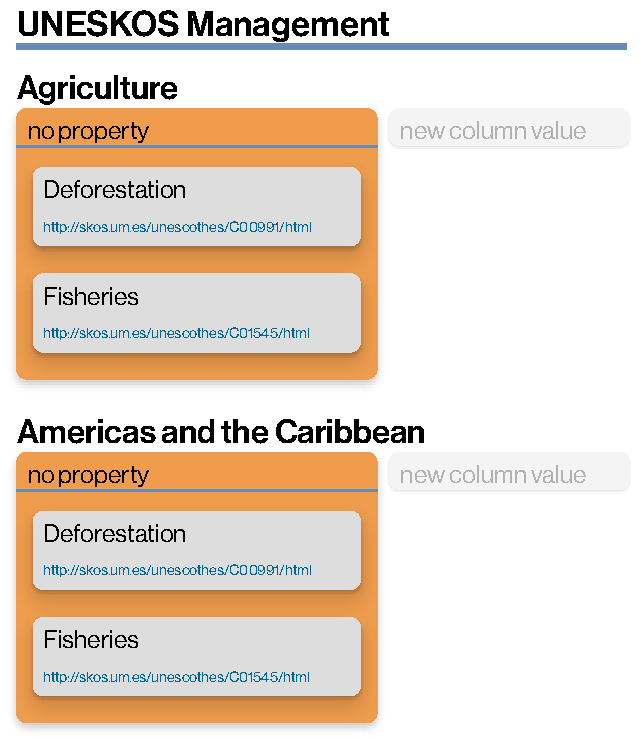
\includegraphics[width=87mm]{img/31-UseCase2.pdf}
	\caption[\tracknshrink{RMB} Mockup of Use Case 2]{\tracknshrink{RMB} Mockup of Use Case 2, showing a board that consists of two lanes, and, due to the lack of the requested column property, a fallback column. The cards only contain their mandatory title and resource identifier. Since the cards have not been moved yet, there is no timestamp depicted.}
	\label{fig:RMB Use Case 2}
	\libertineOsF
\end{figure}



\noindent In this scenario, users can create new column values from scratch and assign resources accordingly. Eventually, when all resources have been allocated, the fallback column would vanish, as it would not hold any resource.